%!TEX root = ../BUSystematics.tex

\graphicspath{{Body/Figures/Pileup/}{Body/Figures/Pileup/Amplitude/}{Body/Figures/Pileup/TimeShift/}{Body/Figures/Pileup/EnergyModel/}{Body/Figures/Pileup/TriplePileup/}{Body/Figures/Pileup/RateError/}}

\section{Pileup}

The pileup correction used in the BU analysis is the asymmetric shadow window method. Extensive details can be found in \refref{phdthesis:2020Kinnaird}; here is given a brief summary. A pileup correction is constructed by looking in ``shadow'' time windows some time after ``trigger'' pulses for trailing shadow pulses. The assumption is that the probability for a pileup event to occur is the same as that to find a shadow pulse trailing a trigger pulse in the right length time window. By looking in all such shadow windows for all trigger pulses and constructing ``shadow doublets,'' a pileup correction is constructed and then applied to the data. The length of the shadow window is called the ``shadow dead time,'' and the gap time between the trigger pulse time and the start of the shadow window is called the ``shadow gap time.''  \tabref{tab:pileupParameters} gives the parameter values for the pileup parameters. The shadow gap time of \ns{10} was chosen to be suitably small such that the event rate was marginally different from the real pileup rate at the trigger pulse time. The shadow dead time of \ns{4.06} was determined by scanning over shadow dead times and finding the value at which the ratio of pileup energies over measured energies in the range \SIrange{3.5}{4.5}{\GeV} was equal to 1, where pileup doublets make up almost the entirety of the counts\footnote{This value of \ns{4.06} is a direct effect of the clustering dead time of 3~cts applied to the Run~1 datasets for ReconWest. With this shadow dead time applied in the procedure, no additional nominal multiplier beyond 1 is applied to the pileup amplitude as was done in the author's dissertation, or other shadow methods.}. On a separate but important note, in the final analysis no local artificial dead time was applied to the incoming clusters. This is in comparison to the analysis done for the dissertation in which an artifical dead time of \ns{5} was applied to the incoming clusters \cite{phdthesis:2020Kinnaird}.


\begin{table}[h]
\centering
% \setlength\tabcolsep{10pt}
\renewcommand{\arraystretch}{1.2}
\begin{tabularx}{0.4\linewidth}{lc}
  \hline
    \multicolumn{2}{c}{\textbf{Pileup Parameters}} \\
  \hline\hline
    Parameter & \thead{Value} \\
  \hline
    Shadow dead time & 4.06~ns \\
    Shadow gap time $(T_{G})$ & 10~ns \\ 
    Pileup energy scaling $(C)$ & 1 \\
  \hline
\end{tabularx}
\caption[]{}
\label{tab:pileupParameters}
\end{table}


The time and energy models for the shadow pileup construction are given as
        \begin{gather}
            E_{\text{doublet}} = C \cdot (E_{\rm T} + E_{\rm S}), \label{eq:Edoublet} \\
            t_{\text{doublet}} = \frac{t_{\rm T} \cdot E_{\rm T} + (t_{\rm S}-T_{G}) \cdot E_{\rm S}}{E_{\rm T} + E_{\rm S}} + \frac{T_{G}}{2}, \label{eq:tdoublet}
        \end{gather}
where $E_{\text{doublet}}$ and $t_{\text{doublet}}$ are the energies and times of the constructed shadow doublets, and $E_{T}$, $E_{S}$, $t_{T}$, $t_{S}$, are the energies and times of the trigger and shadow pulses respectively. $C$ is an energy scaling parameter with a nominal value of 1, and $T_{G}$ is the shadow gap time. The energy of the constructed shadow doublet is simply the sum of the two singlets, while the time is the energy weighted time of the two singlets plus a time-shift of $\frac{T_{G}}{2}$. This time-shift accounts for the fact that combining two pulses with a shift of $T_{G}$ between them is most representative (approximately) of the pileup rate with a time-shift of $T_{G}/2$ on the constructed shadow doublet.


Systematic uncertainties arise primarily from uncertainties in the pileup correction amplitude, as well as the time and energy models used. Others include uncertainties due to the pileup rate, unseen pileup, and the omission of triples in the correction. No systematic uncertainty was evaluated in regards to an artificial dead time since none was applied in the analysis beyond that in the clustering.



\subsection{Amplitude}

The pileup amplitude uncertainty was evaluated by applying multipliers to the amplitude of the pileup correction, and refitting the data. Multipliers were applied in steps of 0.01 from 0.9 to 1.1, and the resulting \R vs pileup multiplier plot was fit to determine the sensitivity of \R to the pileup multiplier. The uncertainty in the multiplier was determined as the width of the parabola in the \chisq vs pileup multiplier plot. The systematic uncertainty on \R was then calculated as 
    \begin{align}
        \delta R = \sigma_{P_{m}} \times \frac{dR}{dP_{m}},
    \end{align}
where $P_{m}$ is the value of the pileup multiplier. \figref{fig:PMscan} shows the scan results for the 9d dataset. \tabref{tab:pileupMultplierScan} show the scan results and \tabref{tab:systematicError_pileupMultplier} gives the systematic uncertainties for each of the Run~1 datasets.





\begin{table}[h]
\centering
% \setlength\tabcolsep{10pt}
\renewcommand{\arraystretch}{1.2}
\begin{tabularx}{0.7\linewidth}{XOOOO}
  \hline
    \multicolumn{5}{c}{\textbf{Pileup Amplitude Scan Results}} \\
  \hline\hline
    Dataset & \thead{Fit Method} & \multicolumn{1}{c}{$dR/dP_{m}$} & \multicolumn{1}{c}{$\sigma_{P_{m}}$} & \multicolumn{1}{c}{$P_{m_{\text{min}}}$} \\
  \hline
    \multirow{2}{*}{60h} & T & $-353.1$ & 0.061 & 0.981 \\
                         & R & $-308.3$ & 0.064 & 1.014 \\
  \hline
    \multirow{2}{*}{HighKick} & T & $-235.2$ & 0.049 & 0.981 \\
                              & R & $-217.0$ & 0.053 & 0.982 \\
  \hline
    \multirow{2}{*}{9d} & T & $-187.8$ & 0.043 & 0.988 \\
                        & R & $-217.6$ & 0.046 & 1.002 \\
  \hline
    \multirow{2}{*}{Endgame} & T & $-326.4$ & 0.031 & 0.879 \\
                             & R & $-269.0$ & 0.035 & 0.958 \\
  \hline
\end{tabularx}
\caption[]{Results for pileup amplitude multiplier scans for the four Run~1 datasets for both fit methods. Include are the sensitivities of \R to the pileup multiplier, uncertainty on the amplitude as determined from the width of the \chisq parabolas, and the pileup multiplier for which the \chisq was a minimum. The sensitivities are in units of ppb per unit multiplier (or just ppb), and the rest of the quantities are unitless.}
\label{tab:pileupMultplierScan}
\end{table}


\begin{table}[h]
\centering
\renewcommand{\arraystretch}{1.2}
\begin{tabularx}{0.6\linewidth}{XYY}
  \hline
    \multicolumn{3}{c}{\textbf{Pileup Amplitude Systematic Uncertainties}} \\
  \hline\hline
    Dataset & \thead{T-Method} & \thead{R-Method} \\
  \hline
    60h & 21.7 & 19.9 \\
    HighKick & 11.4 & 11.4 \\
    9d & 8.1 & 10.1 \\ 
    Endgame & 10.1 & 9.4 \\
  \hline
\end{tabularx}
\caption[]{Systematic uncertainties due to the pileup amplitude. Units are in ppb.}
\label{tab:systematicError_pileupMultplier}
\end{table}


\begin{figure}[h]
\centering
    \begin{subfigure}[t]{0.45\textwidth}
        \centering
        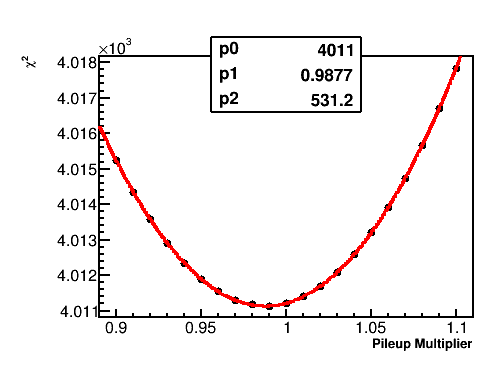
\includegraphics[width=\textwidth]{TMethod_Chi2_Vs_PileupMultiplier_Canv}
        \caption{T-Method \chisq versus pileup multiplier. The parabolic fit equation used was $y = p_{2}(x - p_{1})^{2} + p_{0}.$}
    \end{subfigure}% %you need this % here to add spacing between subfigures
    \hspace{1cm}
    \begin{subfigure}[t]{0.45\textwidth}
        \centering
        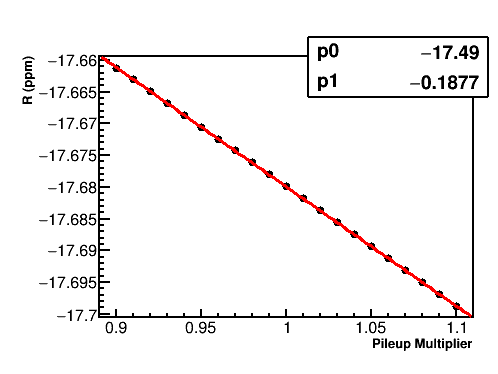
\includegraphics[width=\textwidth]{TMethod_R_Vs_PileupMultiplier_Canv}
        \caption{T-Method $R$ versus pileup multiplier. The parameter $p_{1}$ gives the sensitivity of $R$ to the value of the pileup multiplier, with units in ppm per unit multiplier.}
    \end{subfigure}

    \begin{subfigure}[t]{0.45\textwidth}
        \centering
        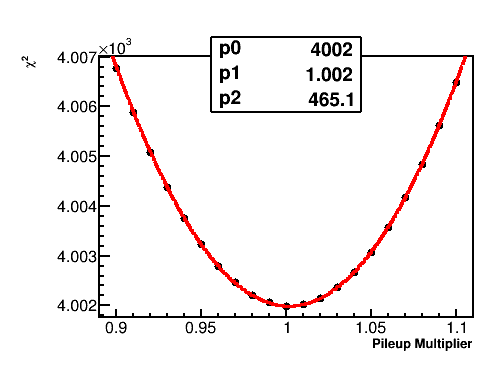
\includegraphics[width=\textwidth]{FullRatio_Chi2_Vs_PileupMultiplier_Canv}
        \caption{R-Method \chisq versus pileup multiplier. The parabolic fit equation used was $y = p_{2}(x - p_{1})^{2} + p_{0}.$}
    \end{subfigure}% %you need this % here to add spacing between subfigures
    \hspace{1cm}
    \begin{subfigure}[t]{0.45\textwidth}
        \centering
        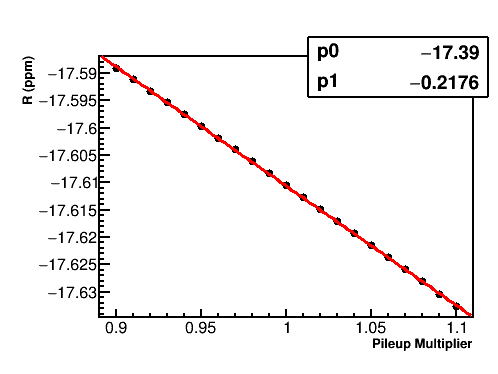
\includegraphics[width=\textwidth]{FullRatio_R_Vs_PileupMultiplier_Canv}
        \caption{R-Method $R$ versus pileup multiplier. The parameter $p_{1}$ gives the sensitivity of $R$ to the value of the pileup multiplier, with units in ppm per unit multiplier.}
    \end{subfigure}
\caption[Pileup multiplier scan]{Pileup multiplier scan. The width of the parabola is determined as the change in X which increases the \chisq by one, which is equal to $1/\sqrt{p_{2}}$. Data are from the 9d dataset.}
\label{fig:PMscan}
\end{figure}



\clearpage
\subsection{Time Model}

The time of a constructed shadow doublet in the pileup construction is set as the energy weighted time of the two singlets plus half the gap time, as shown in \equref{eq:tdoublet}. Previously the uncertainty was calculated by scanning over an additional time-shift parameter and then applying a conservative uncertainty of \ns{2.5} \cite{phdthesis:2020Kinnaird}. The results of such a scan can be seen in \figref{fig:PTSscan}. If this procedure is used then the systematic uncertainty on \R is less than 15~ppb for all datasets. If the most energetic singlet time is set as the doublet time instead, then the $\Delta R$ is less than \ppb{1} for all datasets. Lastly, if the doublet time is set as either the first singlet time, or the second singlet time, then the $\Delta R$'s range approximately from 5--6~ppb, as shown in \tabref{tab:systematicError_clusterTime}. This last approach bounds the possibilities for properly constructed doublet times, and is less conservative than the first approach described, therefore the systematic uncertainty is taken as the average of the absolute values of the two \DR values when using the first and last singlet times. The final systematic uncertainties are also given in \tabref{tab:systematicError_clusterTime} in bold.




\begin{figure}[h]
\centering
    \begin{subfigure}[t]{0.45\textwidth}
        \centering
        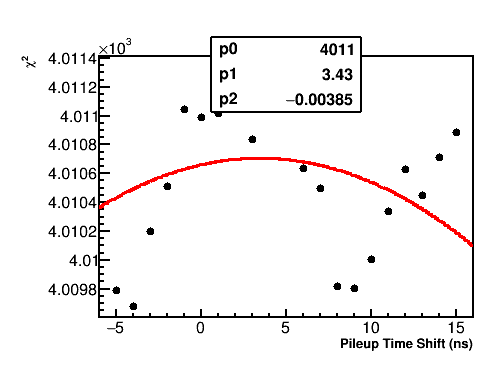
\includegraphics[width=\textwidth]{TMethod_Chi2_Vs_PileupTimeShift_Canv}
        \caption{T-Method \chisq versus pileup time shift. There is no clear parabolic shape or minimum.}
    \end{subfigure}% %you need this % here to add spacing between subfigures
    \hspace{1cm}
    \begin{subfigure}[t]{0.45\textwidth}
        \centering
        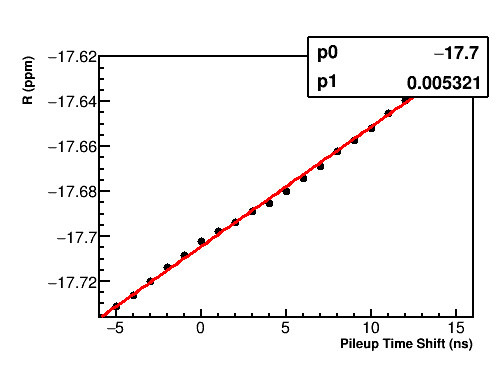
\includegraphics[width=\textwidth]{TMethod_R_Vs_PileupTimeShift_Canv}
        \caption{T-Method $R$ versus pileup time shift. The parameter $p_{1}$ gives the sensitivity of $R$ to the value of the pileup time shift, with units in ppm per ns.}
    \end{subfigure}
\caption[Pileup time shift scan]{Pileup time shift scan for the T-Method. The R-Method plots look the same. There is a wave in the \R plot, but the effect is small and therefore ignored. Data are from the 9d dataset.}
\label{fig:PTSscan}
\end{figure}


\begin{table}[h]
\centering
\renewcommand{\arraystretch}{1.2}
\begin{tabularx}{0.9\linewidth}{@{\extracolsep{\fill}}XHHPHHP}
  \hline
    \multicolumn{7}{c}{Time Model Systematic Uncertainty} \\
  \hline\hline
            & \multicolumn{3}{c}{T-Method} & \multicolumn{3}{c}{R-Method } \\
            \cmidrule(lr){2-4}\cmidrule(lr){5-7}
    Dataset & \thead{First Time} & \thead{Last Time} & \thead{\dR} & \thead{First Time} & \thead{Last Time} & \thead{\dR} \\
  \hline
    60h & -5.5 & 4.6 & 5.1 & -8.0 & 4.8 & 6.4 \\
    HighKick & -5.0 & 4.3 & 4.6 & -5.6 & 4.0 & 4.8 \\
    9d & -5.4 & 5.6 & 5.5 & -5.8 & 5.4 & 5.6 \\ 
    Endgame & -5.5 & 4.4 & 5.0 & -5.2 & 4.3 & 4.8 \\
  \hline
\end{tabularx}
\caption[]{$\Delta R$s when applying either of the two singlet times as the doublet time in the pileup construction, and associated systematic uncertainties calculated as the average of the absolute value of the two values. Units are in ppb.}
\label{tab:systematicError_clusterTime}
\end{table}



% \begin{table}[h]
% \centering
% \renewcommand{\arraystretch}{1.2}
% \begin{tabularx}{0.9\linewidth}{@{\extracolsep{\fill}}XYYYY}
%   \hline
%     \multicolumn{5}{c}{$\Delta R$ with First and Last Singlet Times} \\
%   \hline\hline
%             & \multicolumn{2}{c}{T-Method} & \multicolumn{2}{c}{R-Method } \\
%             \cmidrule(lr){2-3}\cmidrule(lr){4-5}
%     Dataset & \thead{First Time} & \multicolumn{1}{c}{Last Time} & \thead{First Time} & \thead{Last Time}  \\
%   \hline
%     60h & -5.5 & 4.6 & -8.0 & 4.8 \\
%     HighKick & -5.0 & 4.3 & -5.6 & 4.0 \\
%     9d & -5.4 & 5.6 & -5.8 & 5.4 \\ 
%     Endgame & -4.5 & 4.4 & -5.2 & 4.3 \\
%   \hline
% \end{tabularx}
% \caption[]{$\Delta R$ when applying either of the two singlet times as the doublet time in the pileup construction. Units are in ppb.}
% \label{tab:systematicError_clusterTimeDeltas}
% \end{table}





% \begin{table}[h]
% \centering
% \renewcommand{\arraystretch}{1.2}
% \begin{tabularx}{0.5\linewidth}{@{\extracolsep{\fill}}XYY}
%   \hline
%     \multicolumn{3}{c}{\textbf{Time Model Systematic Uncertainty}} \\
%   \hline\hline
%     Dataset & \thead{T-Method} & \thead{R-Method} \\
%   \hline
%     60h & 5.1 & 6.4 \\
%     HighKick & 4.6 & 4.8 \\
%     9d & 5.5 & 5.6 \\ 
%     Endgame & 5.0 & 4.8 \\
%   \hline
% \end{tabularx}
% \caption[]{Systematic uncertainty due to cluster time model. Units are in ppb.}
% \label{tab:systematicError_clusterTimeModel}
% \end{table}





\clearpage
\subsection{Energy Model}

The energy of the shadow doublet in the pileup construction is calculated nominally as the sum of the two singlets, as shown in \equref{eq:Edoublet}. This is an okay approximation as the reconstruction typically assigns the energy of any pileup pulse as such, especially when the spatial separation is turned off as it is in the ReconWest reconstruction. Previously the systematic uncertainty was determined by scanning over the multiplier $C$ on the energy sum from 0.9 to 1.1, taking the slope as the sensitivity, and then multiplying it by the uncertainty determined as in the pileup amplitude systematic uncertainty evaluation (from the width of the \chisq parabola). An example of such a scan is shown in \figref{fig:PESscan}. It was found that the uncertainties as determined from the \chisq ranged from 3--6.4\% depending on the dataset (going smaller with more statistics), with corresponding systematic uncertainties of 5--20~ppb. While some datasets had clear slopes in \R vs the energy scale multplier, some did not.



\begin{figure}[h]
\centering
    \begin{subfigure}[t]{0.45\textwidth}
        \centering
        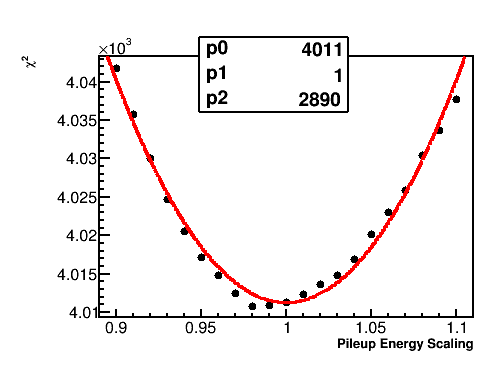
\includegraphics[width=\textwidth]{TMethod_Chi2_Vs_PileupEnergyScaling_Canv}
        \caption{T-Method \chisq versus pileup energy scale. The parabolic fit equation used was $y = p_{2}(x - p_{1})^{2} + p_{0}.$}
    \end{subfigure}% %you need this % here to add spacing between subfigures
    \hspace{1cm}
    \begin{subfigure}[t]{0.45\textwidth}
        \centering
        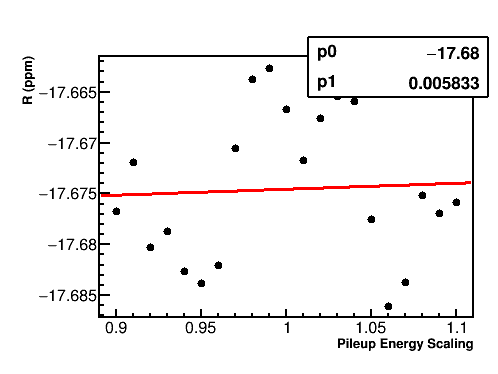
\includegraphics[width=\textwidth]{TMethod_R_Vs_PileupEnergyScaling_Canv}
        \caption{T-Method $R$ versus pileup energy scale. The parameter $p_{1}$ gives the sensitivity of $R$ to the value of the pileup energy scale, with units in ppm per unit scale factor.}
    \end{subfigure}

    \begin{subfigure}[t]{0.45\textwidth}
        \centering
        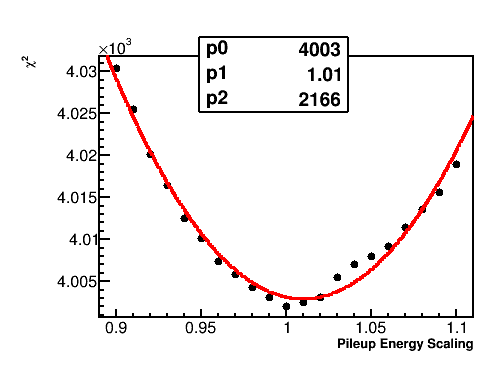
\includegraphics[width=\textwidth]{FullRatio_Chi2_Vs_PileupEnergyScaling_Canv}
        \caption{R-Method \chisq versus pileup energy scale. The parabolic fit equation used was $y = p_{2}(x - p_{1})^{2} + p_{0}.$}
    \end{subfigure}% %you need this % here to add spacing between subfigures
    \hspace{1cm}
    \begin{subfigure}[t]{0.45\textwidth}
        \centering
        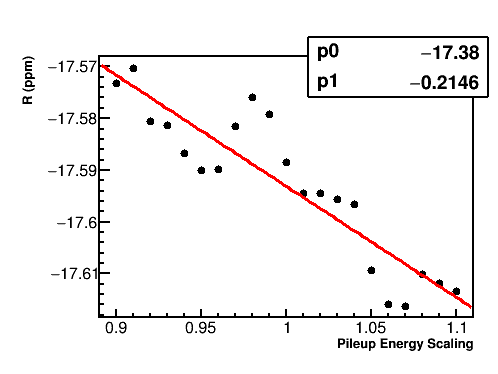
\includegraphics[width=\textwidth]{FullRatio_R_Vs_PileupEnergyScaling_Canv}
        \caption{R-Method $R$ versus pileup energy scale. The parameter $p_{1}$ gives the sensitivity of $R$ to the value of the pileup energy scale, with units in ppm per unit scale factor.}
    \end{subfigure}
\caption[Pileup energy scale scan]{Pileup energy scale scan. Data are from the 9d dataset.}
\label{fig:PESscan}
\end{figure}



Simulations showed however that the energy resolution is much better than that determined by the \chisq; see \figref{fig:ReconEastDoubletEnergyRatios}. Because of this, and because of the non-linear slopes in \R for some datasets, the uncertainty was instead taken as the max $\Delta R$ when applying a $\pm1\%$ scale factor on the doublet energy. This is a reasonable approach, and slightly conservative, as the maximum ratio difference from 1 for energy sums larger than \SI{1.7}{\GeV} is about 1\%. ReconWest is not expected to be significantly different than ReconEast (which was used in the previously mentioned simulations), and the lack of spatial separation would imply that this ratio would be even closer to 1, approximately 0.5\% or so. The systematic uncertainties for the four Run~1 datasets determined via this procedure are given in \tabref{tab:systematicError_clusterEnergyModel}.


\begin{figure}[h]
\centering
    \begin{subfigure}[t]{0.45\textwidth}
        \centering
        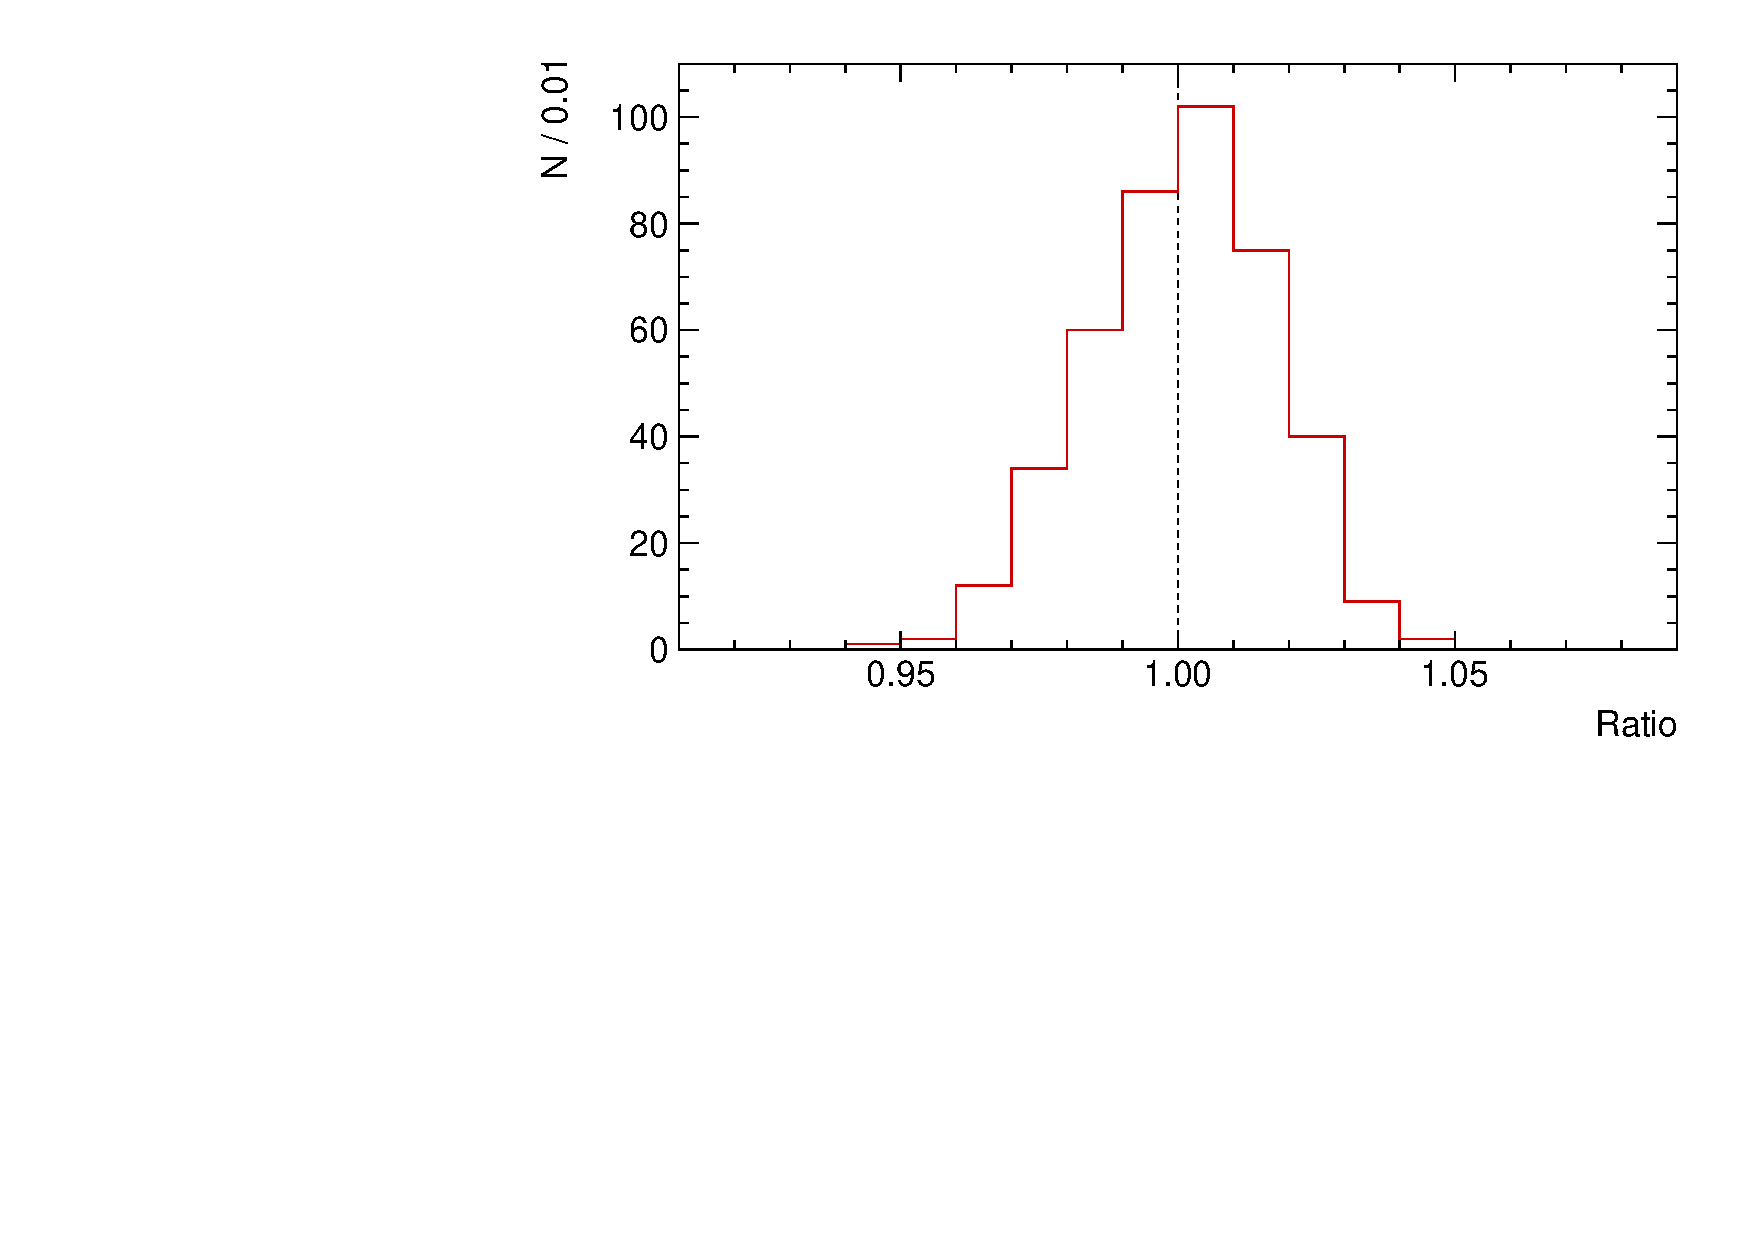
\includegraphics[width=\textwidth]{p_ratio_2_2_hist}
        \caption{The ratio of the doublet energy to the sum of the two singlets for two positrons each with energy 2~\GeV.}
    \end{subfigure}%
    \hspace{1cm}
    \begin{subfigure}[t]{0.45\textwidth}
        \centering
        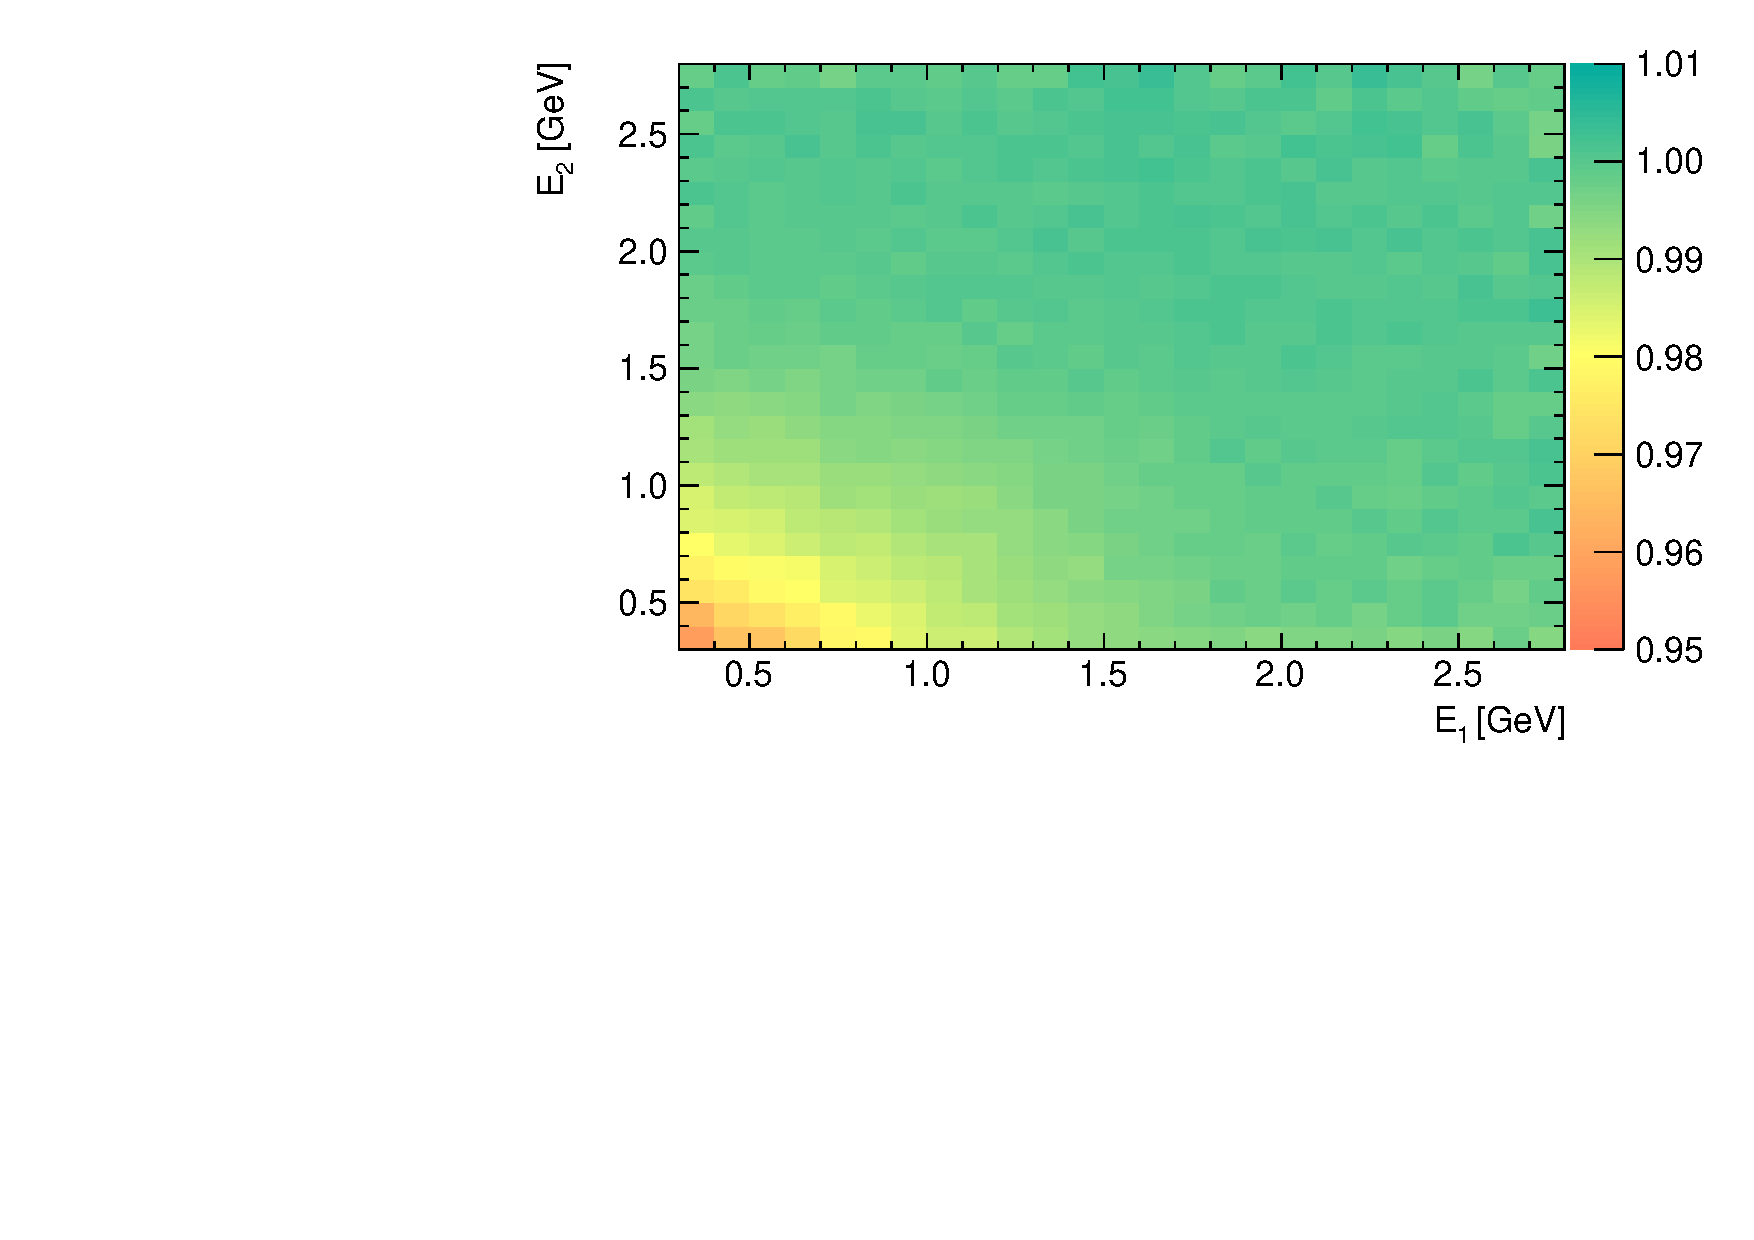
\includegraphics[width=\textwidth]{p_ratio_e1_e2}
        \caption{The average ratio of the doublet energy to the sum of the two singlets as a function of singlet energies.}
    \end{subfigure}
\caption[]{Results from simulations performed by D. Sweigart to determine the ratio of pileup doublet energies to the sum of the two singlets. In the simulations two positrons were fired at the calorimeter using the MDC1 simulation conditions. For cases were pileup occurred, the ratios of the doublet energy to the sum of the two singlets were calculated. The plot on the left is all such energy ratios for the case where the two singlets each had an energy of 2~\GeV, and the plot on the right is the average ratio for all singlet energy combinations. For low energies the ratio can be significantly different from 1, whereas for energies above 1.7~\GeV the difference from 1 is around 1\% or less. Plots courtesy of David Sweigart.}
\label{fig:ReconEastDoubletEnergyRatios}
\end{figure}


\begin{table}[h]
\centering
\renewcommand{\arraystretch}{1.2}
\begin{tabularx}{0.6\linewidth}{@{\extracolsep{\fill}}XYY}
  \hline
    \multicolumn{3}{c}{\textbf{Energy Model Systematic Uncertainty}} \\
  \hline\hline
    Dataset & \thead{T-Method} & \thead{R-Method} \\
  \hline
    60h & 11.0 & 10.9 \\
    HighKick & 4.8 & 7.2 \\
    9d & 6.1 & 10.2 \\ 
    Endgame & 10.0 & 6.8 \\
  \hline
\end{tabularx}
\caption[]{Systematic uncertainty due to cluster energy model. Units are in ppb.}
\label{tab:systematicError_clusterEnergyModel}
\end{table}




\clearpage
\subsection{Pileup Rate Uncertainty}

The pileup rate uncertainty arises from the fact that the pileup is estimated from pulses at times $t$ and $t+SGT$ and then placed at $t+SGT/2$. Ideally the pileup would have been estimated at those latter times from the beginning. There will be differences due to the muon precession and beam dynamics. Because my SGT is very small at \ns{10}, this uncertainty can be expected to be negligible. Using the prescription as outlined in D. Sweigart's thesis \cite{phdthesis:2020Sweigart}, I estimate the pileup rate uncertainty as 

\begin{align}
	\frac{N^{2}(t) - N(t-\frac{SGT}{2})N(t+\frac{SGT}{2})}{N^{2}(t)},
\end{align}
where $N(t)$ is the fit function determined from a T-Method fit to the data. $N^{2}(t)$ is what we wanted to use when constructing the pileup, but $N(t-\frac{SGT}{2})N(t+\frac{SGT}{2})$ is what we actually used. The rate uncertainty is shown in Figures~\ref{fig:pileupRateError} and \ref{fig:pileupRateErrorZoomed}.

There are some interesting features to point out. The pileup rate uncertainty oscillates at \wa and the shape is constant throughout the fill. The black points in the figure come from the nominal fit, where each graph point is calculated and spaced at 149.2/50 ns = 2.984 ns apart. It turns out that there are spikes at the boundaries of the points as defined in the fit function in ROOT. If I fit with 10x the number of points up to 100,000 as shown in the red graph points, the the spikes accordingly shift, and the shape appears to change. This is an effect of the discretization of the points in the ROOT function used to fit the data. The blue points show the average of the black points over a bin width, and as shown lie in line with the red points. Accounting for the discretization then by averaging over the bin width, the pileup rate uncertainty can be determined from the blue curve and is seen to only wander a maximum of 0.005\%, or 0.00005, away from 0. This is a negligible change in the rate, and the systematic uncertainty is thus taken to be 0 ppb for all datasets. Note that even if the maximum of the black curve were to be taken as the rate uncertainty, then it is still less than 0.04\% or 0.0004 and the systematic uncertainty would still be negligible.


\begin{figure}
    \centering
    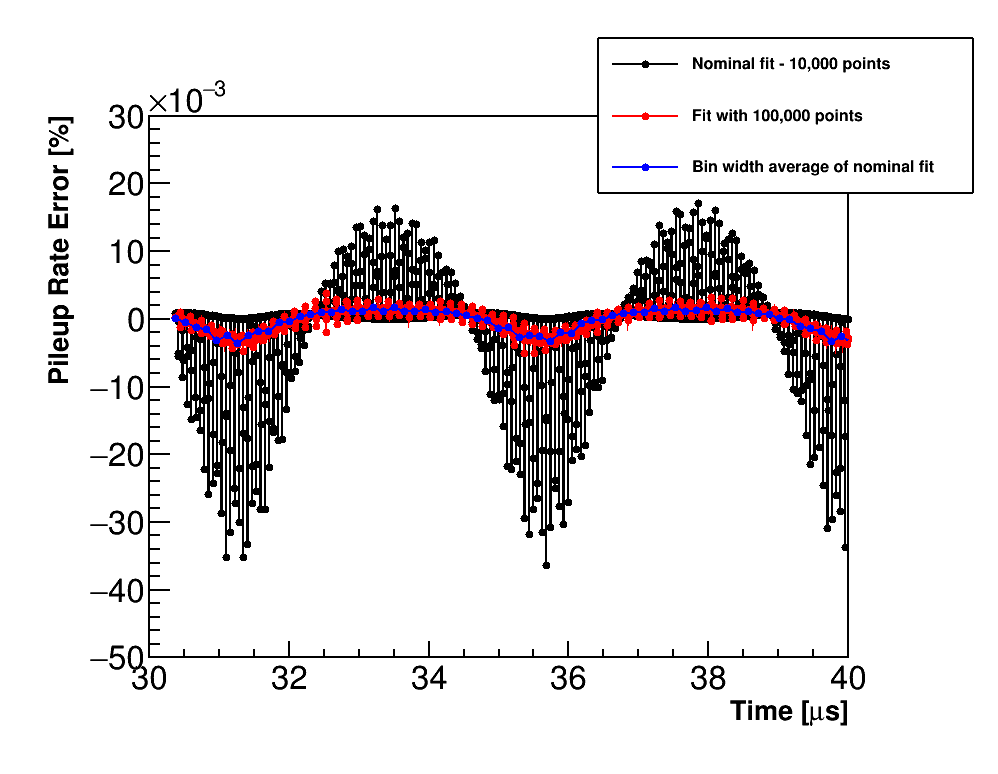
\includegraphics[width=.8\textwidth]{PileupRateError}
    \caption[]{Pileup rate uncertainty. Black points come from the nominal fit, which includes 10,000 points in the ROOT fit function. Red points come from a fit function with 100,000 points, and the blue points are the average of the black points over bin widths. Data are from the 60h dataset.}
    \label{fig:pileupRateError}
\end{figure}

\begin{figure}
    \centering
    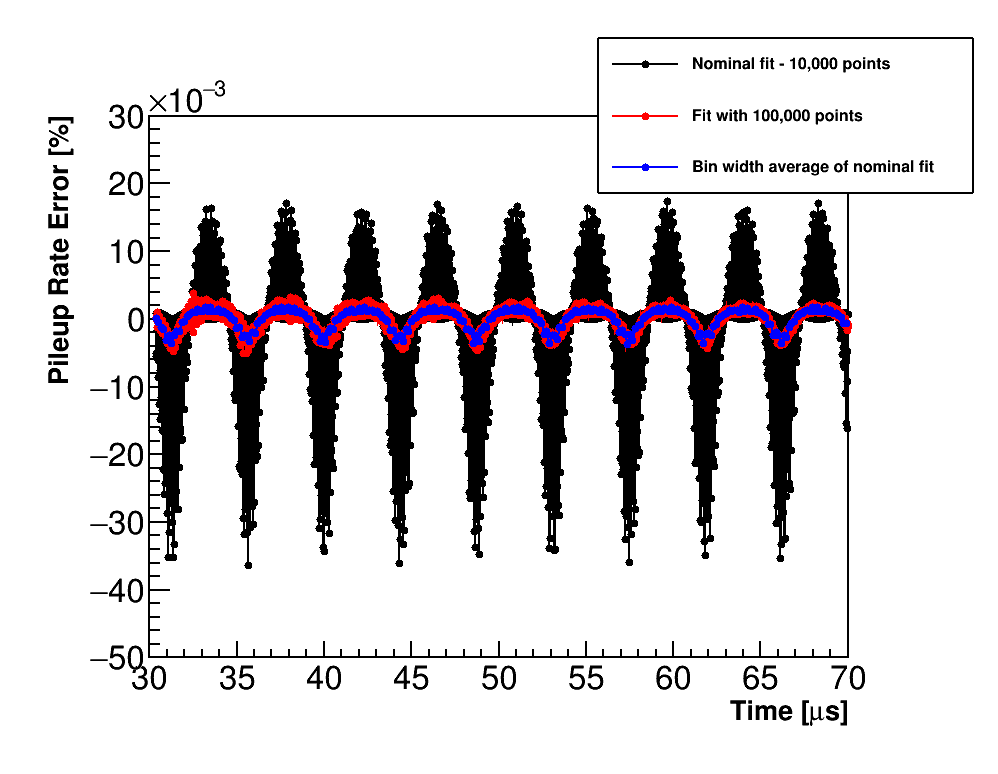
\includegraphics[width=.8\textwidth]{PileupRateError_ZoomedOut}
    \caption[]{The pileup rate uncertainty zoomed out, showing the consistency of the pileup rate uncertainty at later times in the fill. Data are from the 60h dataset.}
    \label{fig:pileupRateErrorZoomed}
\end{figure}

If instead a gap time of \SI{149.2}{\ns} were to be used, the the pileup rate uncertainty is significantly larger as shown in \figref{fig:pileupRateErrorLarger}, oscillating between -0.7\% and 0.3\%. This plot is comparable to David's thesis plot 6.28. Note that spikes can still be seen in the function however due to the discretization, though the relative size of them is much smaller than the rest of the curve.


\begin{figure}
    \centering
    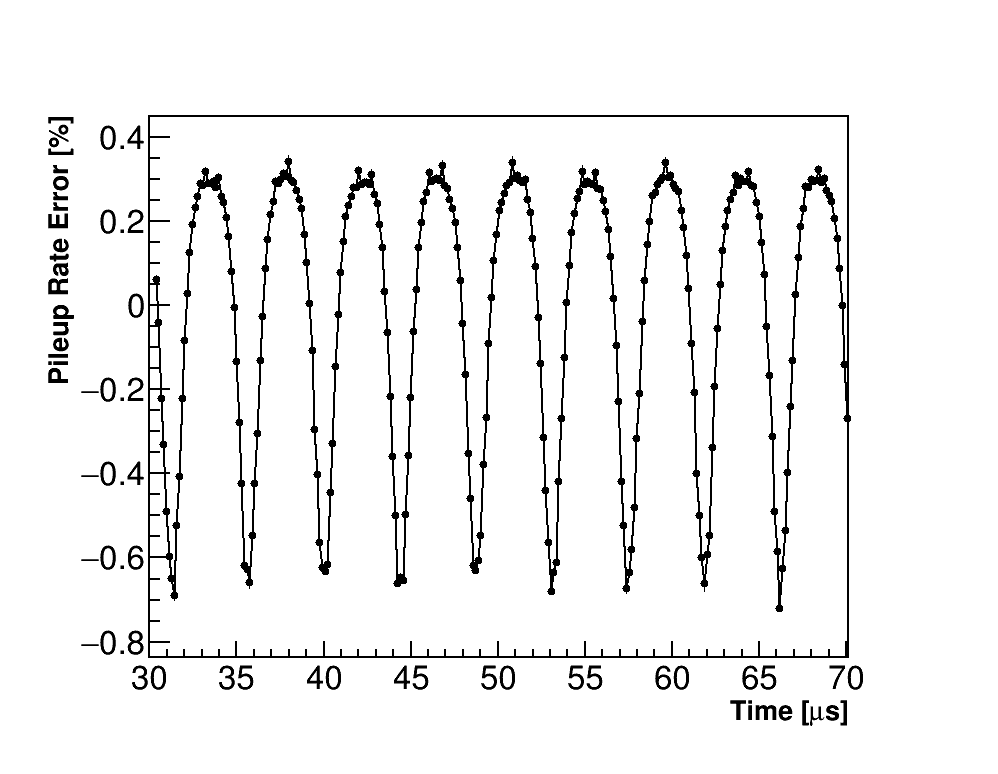
\includegraphics[width=.8\textwidth]{PileupRateError_149p2SGT}
    \caption[]{Pileup rate uncertainty when using a gap time of \SI{149.2}{\ns}. Data are from the 60h dataset.}
    \label{fig:pileupRateErrorLarger}
\end{figure}




\clearpage
\subsection{Unseen Pileup}

The systematic uncertainty due to unseen pileup is given in \tabref{tab:systematicError_unseenPileup}. They are calculated by ignoring pileup pulses below \SI{100}{\MeV} in the pileup construction, a value which twice as high as the expected missed pulse energies of around \SI{50}{\MeV} or less. If the threshold is raised to \SI{200}{\MeV} then the systematic uncertainties range around in the ballpark from 10-30 ppb.

\begin{table}
\centering
\renewcommand{\arraystretch}{1.2}
\begin{tabularx}{0.65\linewidth}{@{\extracolsep{\fill}}XYY}
  \hline
    \multicolumn{3}{c}{\textbf{Systematic Uncertainty due to Unseen Pileup}} \\
  \hline\hline
    Dataset & \thead{T-Method} & \thead{R-Method} \\
  \hline
    60h & 0.8 & 0.6 \\
    HighKick & 1.3 & 0.1 \\
    9d & 2.5 & 2.5 \\ 
    Endgame & 4.1 & 2.4 \\
  \hline
\end{tabularx}
\caption[]{Systematic uncertainty due to unseen pileup. Units are in ppb.}
\label{tab:systematicError_unseenPileup}
\end{table}



\clearpage
\subsection{Triple Pileup Correction}

Triple pileup is not included in my pileup correction. The systematic uncertainty for ignoring the triples is estimated by looking at the $\Delta R$ with and without the doubles correction (which can be gotten from the slopes of the pileup multiplier scans extrapolated to 0, \tabref{tab:pileupMultplierScan}), multiplied against the rate of triples to doubles. The latter can be approximated by the rate of doubles to singles, a plot of which is given in \figref{fig:pileupRateFraction}. As shown the fraction of the pileup is less than 1\% and decreases throughout the fill. The rate is averaged over the first \gmtwo period in the fit before multiplying against the $\Delta R$, the values are given in \tabref{tab:pileupRates}. The systematic uncertainties are given in \tabref{tab:systematicError_triplePileupCorrection}. Even these small numbers here are conservative since the rate drops throughout the fill, and would drop even faster for triples to doubles.


\begin{figure}[h]
    \centering
    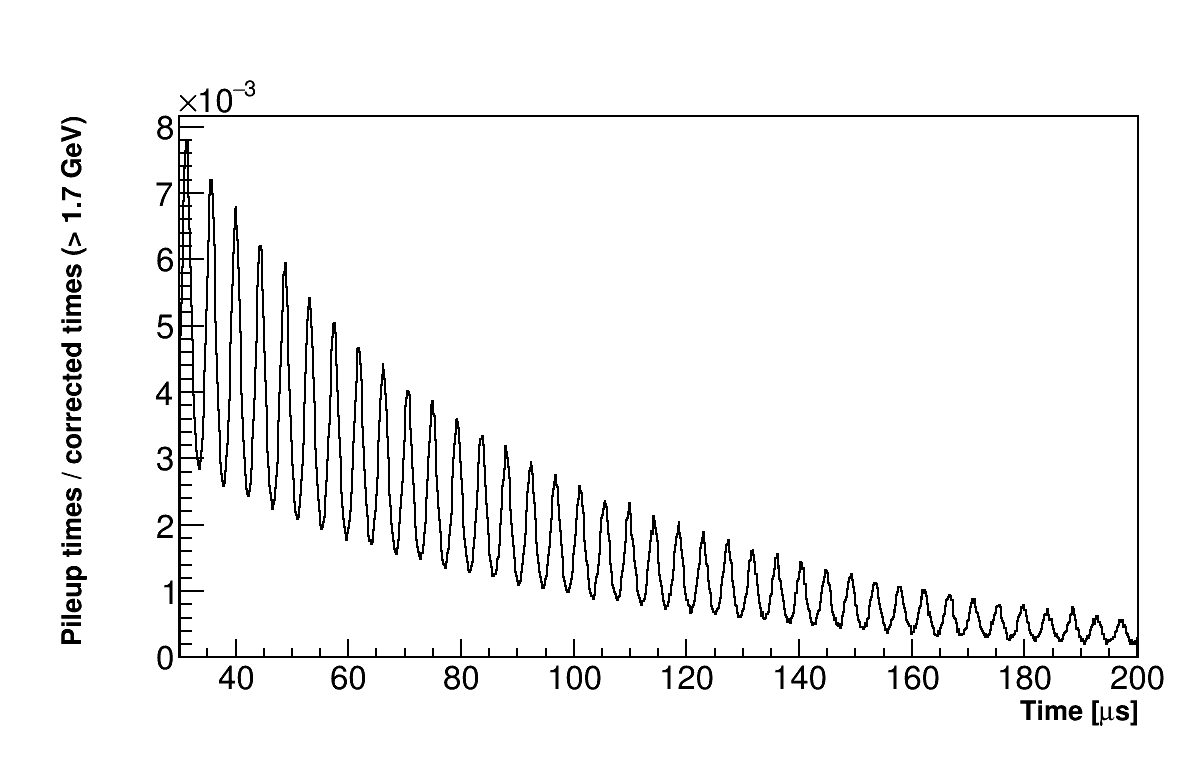
\includegraphics[width=1\textwidth]{pileupRateFraction}
    \caption[]{Pileup rate fraction plot. Data from the Endgame dataset.}
    \label{fig:pileupRateFraction}
\end{figure}


\begin{table}[h]
\centering
\renewcommand{\arraystretch}{1.2}
\begin{tabularx}{0.65\linewidth}{@{\extracolsep{\fill}}lcc}
  \hline
    \multicolumn{3}{c}{\textbf{Pileup Rates}} \\
  \hline\hline
    Dataset & Average rate & Max rate \\
  \hline
    60h & \num{5.33e-3} & \num{8.50e-3} \\
    HighKick & \num{5.69e-3} & \num{8.96e-3} \\
    9d & \num{5.19e-3} & \num{8.32e-3} \\ 
    Endgame & \num{4.93e-3} & \num{7.78e-3} \\
  \hline
\end{tabularx}
\caption[]{Pileup rates over the first \gmtwo period of the fitting range, averaged and the maximum value respectively.}
\label{tab:pileupRates}
\end{table}


\begin{table}[h]
\centering
\renewcommand{\arraystretch}{1.2}
\begin{tabularx}{0.75\linewidth}{@{\extracolsep{\fill}}XYY}
  \hline
    \multicolumn{3}{c}{\textbf{Systematic Uncertainty due to Triple Pileup Correction}} \\
  \hline\hline
    Dataset & \thead{T-Method} & \thead{R-Method} \\
  \hline
    60h & 1.9 & 1.6 \\
    HighKick & 1.3 & 1.2 \\
    9d & 1.0 & 1.1 \\ 
    Endgame & 1.6 & 1.3 \\
  \hline
\end{tabularx}
\caption[]{Systematic uncertainty due to triple pileup correction. Units are in ppb.}
\label{tab:systematicError_triplePileupCorrection}
\end{table}



